\documentclass[10pt,a4paper]{article}
\usepackage[utf8]{inputenc}
\usepackage[ngerman]{babel}
\usepackage[T1]{fontenc}
\usepackage{amsmath}
\usepackage{amsfonts}
\usepackage{amssymb}
\usepackage{graphicx}
\usepackage{lmodern}
\usepackage{physics}
\usepackage[left=1cm,right=1cm,top=1.5cm,bottom=1.2cm]{geometry}
\usepackage{siunitx}
\usepackage{fancyhdr}
\usepackage{enumerate}
\usepackage{mhchem}
\usepackage{mathtools}
\usepackage{graphicx}
\usepackage{float}
\usepackage{xcolor}
\usepackage{mdframed}
\usepackage{csquotes}
\usepackage{trfsigns}
\usepackage{capt-of}

\sisetup{locale=DE}
\sisetup{per-mode = symbol-or-fraction}
\sisetup{separate-uncertainty=true}
\DeclareSIUnit\year{a}
\DeclareSIUnit\clight{c}
\mdfdefinestyle{exercise}{
	backgroundcolor=black!10,roundcorner=8pt,hidealllines=true,nobreak
}

\begin{document}
\twocolumn
\pagestyle{fancy}
\lhead{DSV Formelsammlung}
\rhead{Sedlmeier, Toni}
\section{Elementare DSV}
%%%%%%%%%%%%%%%%%%%%%%%%%%%%%%%%%%%%%%%%%%%%% Energie %%%%%%%%%%%%%%%%%%%%%%%%%%%%%%%%%%%%%%%%%%%%%%%%%%%%%
  \subsection{Energie}
  Die Leistung und Energie eines Signals $x(k)$ $k \in [k_1,k_2]$
  \begin{mdframed}[style=exercise]
    \begin{align}
        E_{k_1,k_2} &=\sum_{k=k_1}^{k_2} \abs{x(k)}^2 \ = (k_2 - k_1 +1) P_{k_1,k_2} 
    \end{align}
  \end{mdframed}
  Parsevallsche Gleichung ZDFT:
  \begin{mdframed}[style=exercise]
    \begin{align}
        E_{-\infty,\infty} &=\sum_{-\infty}^{\infty} \abs{x(k)}^2 = \frac{1}{2\pi}\displaystyle\int_{-\pi}^{\pi} \abs{X(e^{j\Omega})}^2 d\Omega
    \end{align}
  \end{mdframed}
  Parsevallsche Gleichung DFT:
  \begin{mdframed}[style=exercise]
    \begin{align}
        E &=\sum_{k=0}^{N-1} \abs{x(k)}^2 =\frac{1}{N}\sum_{n=0}^{N-1} \abs{X(n)}^2 
    \end{align}
  \end{mdframed}
  \subsection{DFT/IDFT}
  \begin{mdframed}[style=exercise]
    \begin{align}
        X(n)&=\sum_{k=0}^{N-1} x(k)e^{-j\frac{2\pi kn}{N}} \\
        x(k)&=\frac{1}{N}\sum_{n=0}^{N-1} X(n)e^{-j\frac{2\pi kn}{N}} 
    \end{align}
  \end{mdframed}
%%%%%%%%%%%%%%%%%%%%%%%%%%%%%%%%%%%%%%%%%%%%%%%%%%%%%%%%%%%%%%%%%%%%%%%%%%%%%%%%%%%%%%%%%%%%%%%%%%%%%%%%%%%%%%%
%%%%%%%%%%%%%%%%%%%%%%%%%%%%%%%%%%%%% DFT-Korrespondenzen %%%%%%%%%%%%%%%%%%%%%%%%%%%%%%%%%%%%%%%%%%%%%%%%%%%%%
% Fehler mit scale
\scalebox{0.85}{
    \begin{center}
    \begin{tabular}{ c c c }
        & Zeitbereich & Spektralbereich \\
        Linearität & $a\cdot x_1(k) b\cdot x_2(k)$ & $a\cdot X_1(n) +b\cdot X_2(n)$ \\
        Zeit-Verschiebung & $x(k\textcolor{red}{-}k_0)$ & $e^{\textcolor{red}{-}j\frac{2\pi nk_0}{N}} X(n)$\\
        Frequenz-Verschiebung & $e^{\textcolor{red}{-}j\frac{2\pi nk_0}{N}} x(k)$ & $X(n\textcolor{red}{+}k_0)$ \\  
        Spiegelung & $x(-k)$ & $X(-n)$ \\  
        Konj.Kompl & $x^*(k)$& $X^*(-n)$\\ 
        Faltung & $x_1(k) \circledast x_2(k)$ & $X_1(n)X_2(n)$ \\  
        Multiplikation & $x_1(k)x_2(k)$ & $\frac{1}{N} X_1(n) \circledast X_2(n)$ \\
        gerade Symmetrie & $x_g(k)=\frac{x(k)+x(-k)}{2}$ & $X_g(n)=\frac{X(n)+X(-n)}{2}$ \\
        ungerade Symmetrie & $x_u(k)=\frac{x(k)-x(-k)}{2}$ & $X_u(n)=\frac{X(n)-X(-n)}{2}$
    \end{tabular}
    \end{center}
}
%%%%%%%%%%%%%%%%%%%%%%%%%%%%%%%%%%%%%%%%%%%%%%%%%%%%%%%%%%%%%%%%%%%%%%%%%%%%%%%%%%%%%%%%%%%%%%%%%%%%%%%%%%%%
%%%%%%%%%%%%%%%%%%%%%%%%%%%%%%%%%%%%% z-Transformation %%%%%%%%%%%%%%%%%%%%%%%%%%%%%%%%%%%%%%%%%%%%%%%%%%%%%
  \subsection{z-Transformation}
  \begin{mdframed}[style=exercise]
    \begin{align}
        X(z) &=\sum_{k=-\infty}^{\infty} x(k)z^{-k} \ \ z=e^{s T_a}
    \end{align}
  \end{mdframed}
%%%%%%%%%%%%%%%%%%%%%%%%%%%%%%%%%%%%%%%%%%%%%%%%%%%%%%%%%%%%%%%%%%%%%%%%%%%%%%%%%%%%%%%%%%%%%%%%%%%%%%%%%%%%
%%%%%%%%%%%%%%%%%%%%%%%%%%%%%%%%%%%%% z-Korrespondenzen %%%%%%%%%%%%%%%%%%%%%%%%%%%%%%%%%%%%%%%%%%%%%%%%%%%%
  \begin{center}
      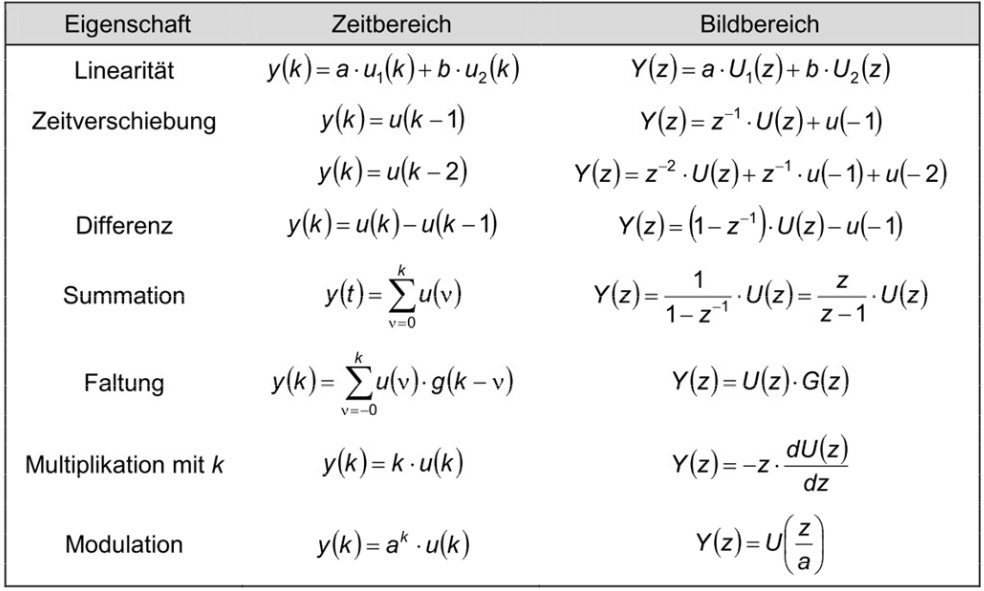
\includegraphics[width=.35\textwidth]{./img/z.png}
  \end{center}
%%%%%%%%%%%%%%%%%%%%%%%%%%%%%%%%%%%%%%%%%%%%%%%%%%%%%%%%%%%%%%%%%%%%%%%%%%%%%%%%%%%%%%%%%%%%%%%%%%%%%%%%%%%%
%%%%%%%%%%%%%%%%%%%%%%%%%%%%%%%%%%%%%%%%%% Faltung %%%%%%%%%%%%%%%%%%%%%%%%%%%%%%%%%%%%%%%%%%%%%%%%%%%%%%%%%
  \subsection{Faltung}
  \subsubsection{Lineare Faltung}
  \begin{mdframed}[style=exercise]
    \begin{align}
        g(k)*u(k) = \sum_{\nu =0}^{k} g(\nu) u(k-\nu)= \sum_{\nu =0}^{k} g(k-\nu) u(\nu)
    \end{align}
  \end{mdframed}
  \subsubsection{Zyklische Faltung}
  $x_1(k)$ und $x_2(k)$ durch \textbf{Zero-Padding} auf $N = N_1 +N_2 -1$ 
  \begin{mdframed}[style=exercise]
    \begin{align}
        x_1(k) \circledast x_2(k) = \sum_{\nu =k_0}^{k_0+N-1} x_1(\nu) x_2(k-\nu)
    \end{align}
  \end{mdframed}
%%%%%%%%%%%%%%%%%%%%%%%%%%%%%%%%%%%%%%%%%%%%%%%%%%%%%%%%%%%%%%%%%%%%%%%%%%%%%%%%%%%%%%%%%%%%%%%%%%%%%%%%%%%%
%%%%%%%%%%%%%%%%%%%%%%%%%%%%%%%%%%%%% Korrelation %%%%%%%%%%%%%%%%%%%%%%%%%%%%%%%%%%%%%%%%%%%%%%%%%%%%%%%%%%
  \subsection{Korrelation}
  $x_1(k) \in [0,N_1-1]$ und $x_2(k) \in [0,N_2-1]$
  \begin{mdframed}[style=exercise]
    \begin{align}
        r_{x1x2}(\lambda) = \sum_{k=-\infty}^{\infty}x_1^*(k) x_2(k+\lambda) 
    \end{align}
  \end{mdframed}
%%%%%%%%%%%%%%%%%%%%%%%%%%%%%%%%%%%%%%%%%%%%%%%%%%%%%%%%%%%%%%%%%%%%%%%%%%%%%%%%%%%%%%%%%%%%%%%%%%%%%%%%%%
%%%%%%%%%%%%%%%%%%%%%%%%%%%%%%%%%%%%% Blocksignalverarbeitung %%%%%%%%%%%%%%%%%%%%%%%%%%%%%%%%%%%%%%%%%%%%
  \subsection{Blocksignalverarbeitung}
  Der $i$-te Block $x^{(i)}(k)$ der Länge $L$ mit Versch.abstand $D$ 
  wird als Multiplikation mit Fensterfunktion $w(k)$ beschrieben
  \begin{mdframed}[style=exercise]
    \begin{align}
        Allg.:
        x^{(i)}(k) = x(k+(i-1)D) \cdot w(k)\ \ k\in[0,L-1] 
    \end{align}
  \end{mdframed}
  Überlapp $D_\%$
  \begin{mdframed}[style=exercise]
    \begin{align}
        D_\% = \frac{L-D}{L}100\%
    \end{align}
  \end{mdframed}
% Overlapp-Add
  \subsubsection{Overlapp-Add Verfahren}
  Schnelle Faltung $g(k)*u(k)$ $N_u >> N_g$ 
  Aufteilung $u(k)$ nicht-überlappend (\textbf{nahtlos}) $\rightarrow D=L$ \\
  Zero-Padding $u^{(i)}(k)$ auf $N=L+N_g$ 
% Overlapp-Save
  \subsubsection{Overlapp-Save Verfahren}
  Schnelle Faltung $g(k)*u(k)$ $N_u >> N_g$ \\
  z.B Überlapp = $N_g-1 \rightarrow D=L-N_g+1$ \\
  \begin{mdframed}[style=exercise]
    \begin{align}
        u^{(i)}(k) = u(k+(i-1)D) \ \ k\in[0,L-1]
    \end{align}
  \end{mdframed}
%%%%%%%%%%%%%%%%%%%%%%%%%%%%%%%%%%%%%%%%%%%%%%%%%%%%%%%%%%%%%%%%%%%%%%%%%%%%%%%%%%%%%%%%%%%%%%%%%%%%%%%%%%
%%%%%%%%%%%%%%%%%%%%%%%%%%%%%%%%%%%%% Simultane Transformation %%%%%%%%%%%%%%%%%%%%%%%%%%%%%%%%%%%%%%%%%%%
  \subsection{Simultane Transformation}
  \begin{mdframed}[style=exercise]
    \begin{align}
        x_1(k) = Re[y(k)] = \frac{1}{2}(y(k)+y^*(k))\\
        x_2(k) = Im[y(k)] = \frac{1}{2j}(y(k)-y^*(k))\\
        x_1(k) = x(2k)\\
        x_2(k) = x(2k+1)\\
        y(k) = x_1(k) +jx_2(k)
    \end{align}
  \end{mdframed}
  \begin{mdframed}[style=exercise]
    \begin{align}
        X_1(n) = \frac{1}{2}(Y(n)+Y^*(-n))\\
        X_2(n) = \frac{1}{2j}(Y(n)-Y^*(n))
    \end{align}
  \end{mdframed}
\end{document}
